\section{A Common Compiler Architecture}
\label{sec:architecture}

\begin{figure}[t]
  \centering
  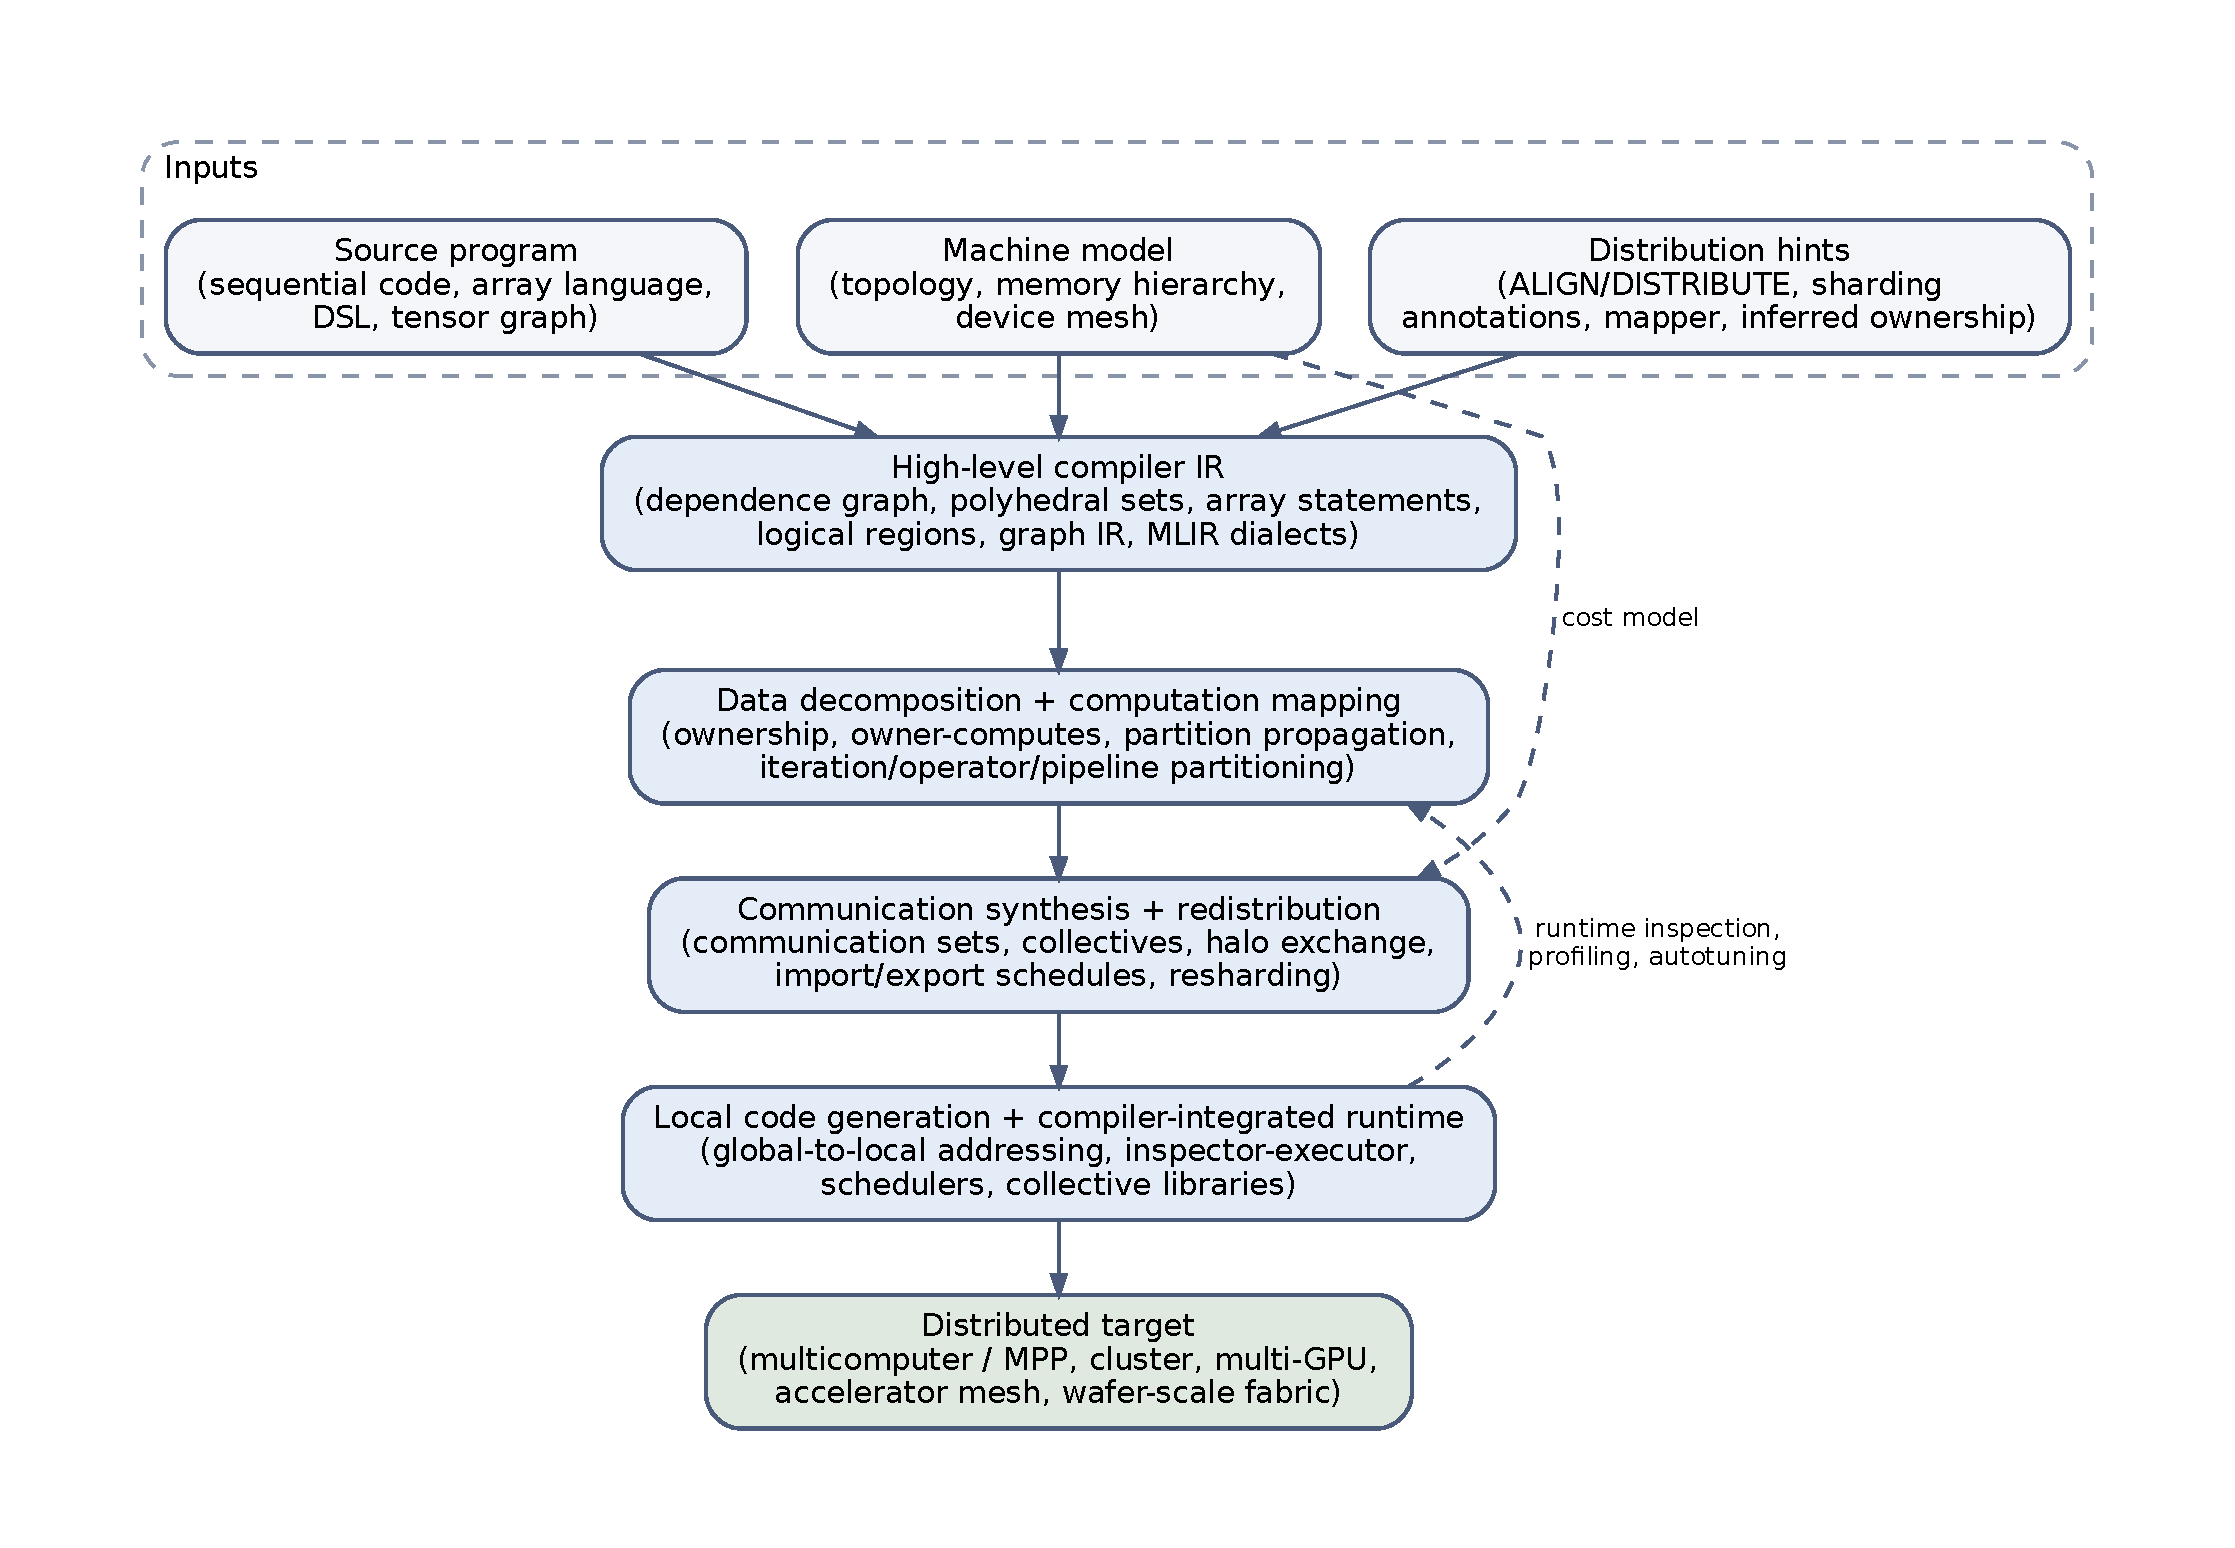
\includegraphics[width=\columnwidth]{compiler-architecture.pdf}
  \caption{The stages that recur across distributed-memory compilers from SUPERB to Shardy. The pipeline is linear in most 1990s systems; the dashed feedback edges (runtime inspection, profiling, autotuning, and cost models) are where the compiler/runtime boundary (axis~F) is drawn differently by different systems. Figure original to this survey; stages are abstracted from the catalog entries cited in the text.}
  \label{fig:architecture}
\end{figure}

\ours{We abstract the systems in the catalog into the pipeline of Fig.~\ref{fig:architecture}.} Its inputs are a source program (sequential code, an array language, a DSL, or an operator graph), a machine model (processor arrangement, device mesh, memory hierarchy, topology), and distribution information that is either supplied (ALIGN/DISTRIBUTE directives~\cite{loveman1993hpf}, sharding annotations~\cite{xu2021gspmd}, a mapper interface~\cite{bauer2012legion}) or inferred.

\paragraph{High-level IR}
\fact{Era-2 compilers worked on dependence graphs over Fortran loops~\cite{hiranandani1992compiling}; polyhedral systems represent iteration and data spaces as integer sets~\cite{bondhugula2013compiling}; ML systems use operator graphs~\cite{xu2021gspmd}; and recent work uses MLIR dialects that carry sharding or distribution attributes~\cite{bisbas2024shared,alabed2025partir}.}

\paragraph{Data decomposition and computation mapping}
\fact{The owner-computes rule, which assigns a statement to the place that owns its left-hand side, appears in the Kali and Fortran~D compilers~\cite{koelbel1991compiling,hiranandani1992compiling}; GSPMD's partition propagation infers shardings of unannotated tensors from annotated ones~\cite{xu2021gspmd}.} \infer{Both are instances of deriving a computation mapping from a data mapping; Section~\ref{sec:mapping} examines the alternatives.}

\paragraph{Communication synthesis and redistribution}
\fact{Compilers derive communication either in closed form from the distribution functions (communication sets and local address generation~\cite{koelbel1991regular,chatterjee1993generating,stichnoth1994generating}), by recognising collective patterns, or at runtime by inspecting indices~\cite{saltz1990runtime}.} Redistribution between phases is a separate stage in HPF compilers~\cite{ramaswamy1996redistribution} and reappears as resharding in SPMD partitioners.

\paragraph{Local code generation and compiler-integrated runtime}
\fact{Era-2/3 compilers emitted SPMD Fortran with calls to message-passing libraries; PARTI/CHAOS supplied runtime schedules for irregular accesses~\cite{das1994communication}; Legion executes a mapped task graph on a runtime that manages region coherence~\cite{bauer2012legion}; XLA-based systems lower to per-device programs with collective calls~\cite{xu2021gspmd}.} \ours{We use the amount of work delegated to the runtime as axis~F of the taxonomy.}

\paragraph{Synthesis}
\infer{The pipeline has been stable since the early 1990s; what has changed across eras is (i) the input abstraction, (ii) the representation on which decomposition is decided, and (iii) which stages are static versus dynamic.} These three differences are exactly axes~B, K, and F of the taxonomy.
